%3. Разработка программного обеспечения
%3.1 Функциональная структура ПО (юскейсы)
\section{Розробка програмного забеспечення}
\subsection{Функціональна структура ПЗ}
\begin{stdfigure}
    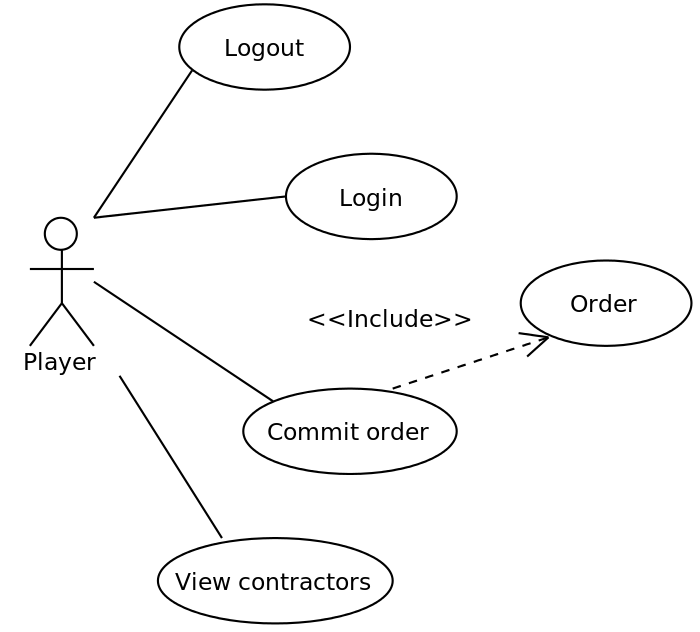
\includegraphics[width=4in]{images/uml/player_use_cases.png}
    \caption{Діаграма використання гравця}
    \label{fig:uml_pl_uc}
\end{stdfigure}   

\begin{stdfigure}
    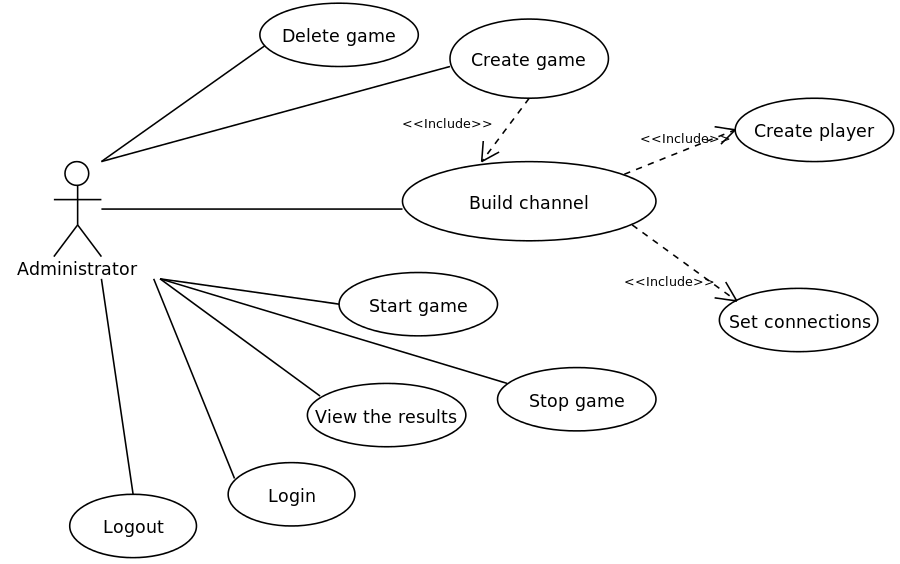
\includegraphics[width=6in]{images/uml/admin_use_cases.png}
    \caption{Діаграма використання адміністратора}
    \label{fig:uml_admin_uc}
\end{stdfigure}   


%3.4 Инструкция пользователю (описать с экранными формами как надо работать с программой)

\subsection{Інформаційно-логічна схема даних}
%3.2 Информационно-логическая схема данных (ЕР модель)
\begin{stdfigure}
    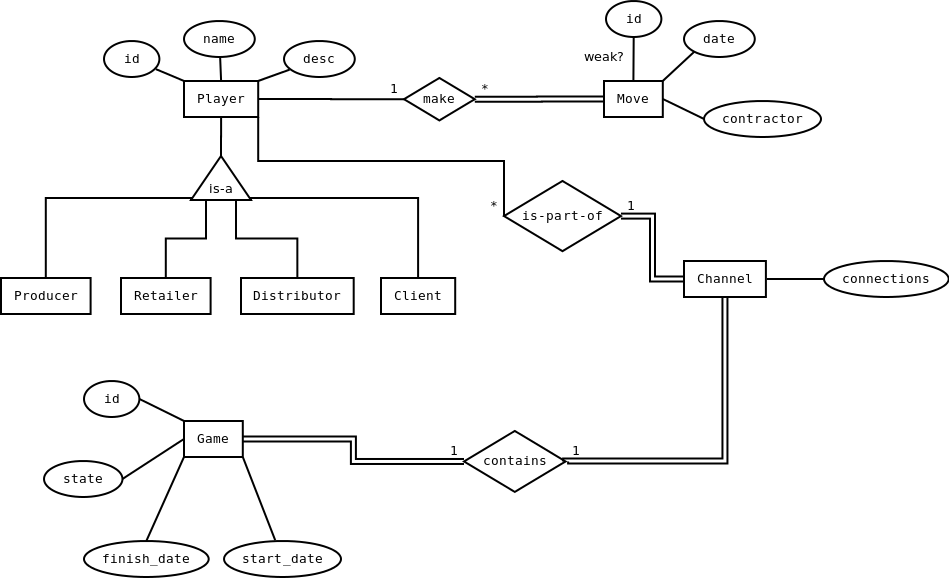
\includegraphics[width=7in]{images/er.png}
    \caption{Логічна модель даних}
    \label{fig:er}
\end{stdfigure}   
\begin{stdfigure}
    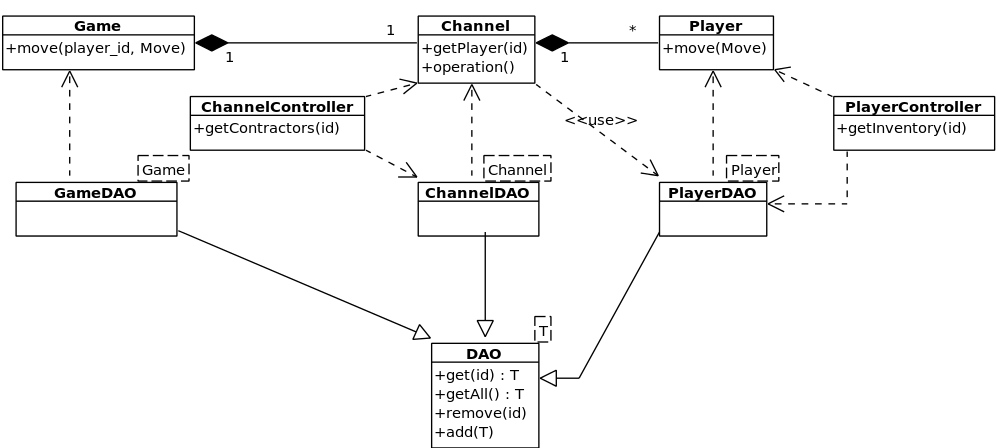
\includegraphics[width=7in]{images/uml/management_level.png}
    \caption{Діаграма класів Management Level}
    \label{fig:uml_management}
\end{stdfigure}   

\begin{stdfigure}
    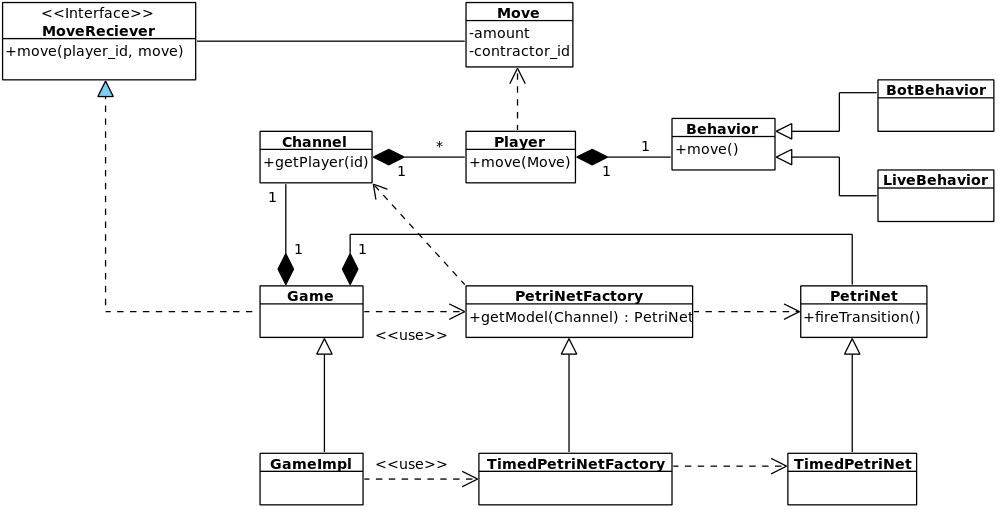
\includegraphics[width=7in]{images/uml/simulation_level.png}
    \caption{Діаграма класів Simulation Level}
    \label{fig:uml_simulation}
\end{stdfigure}   

\begin{stdfigure}
    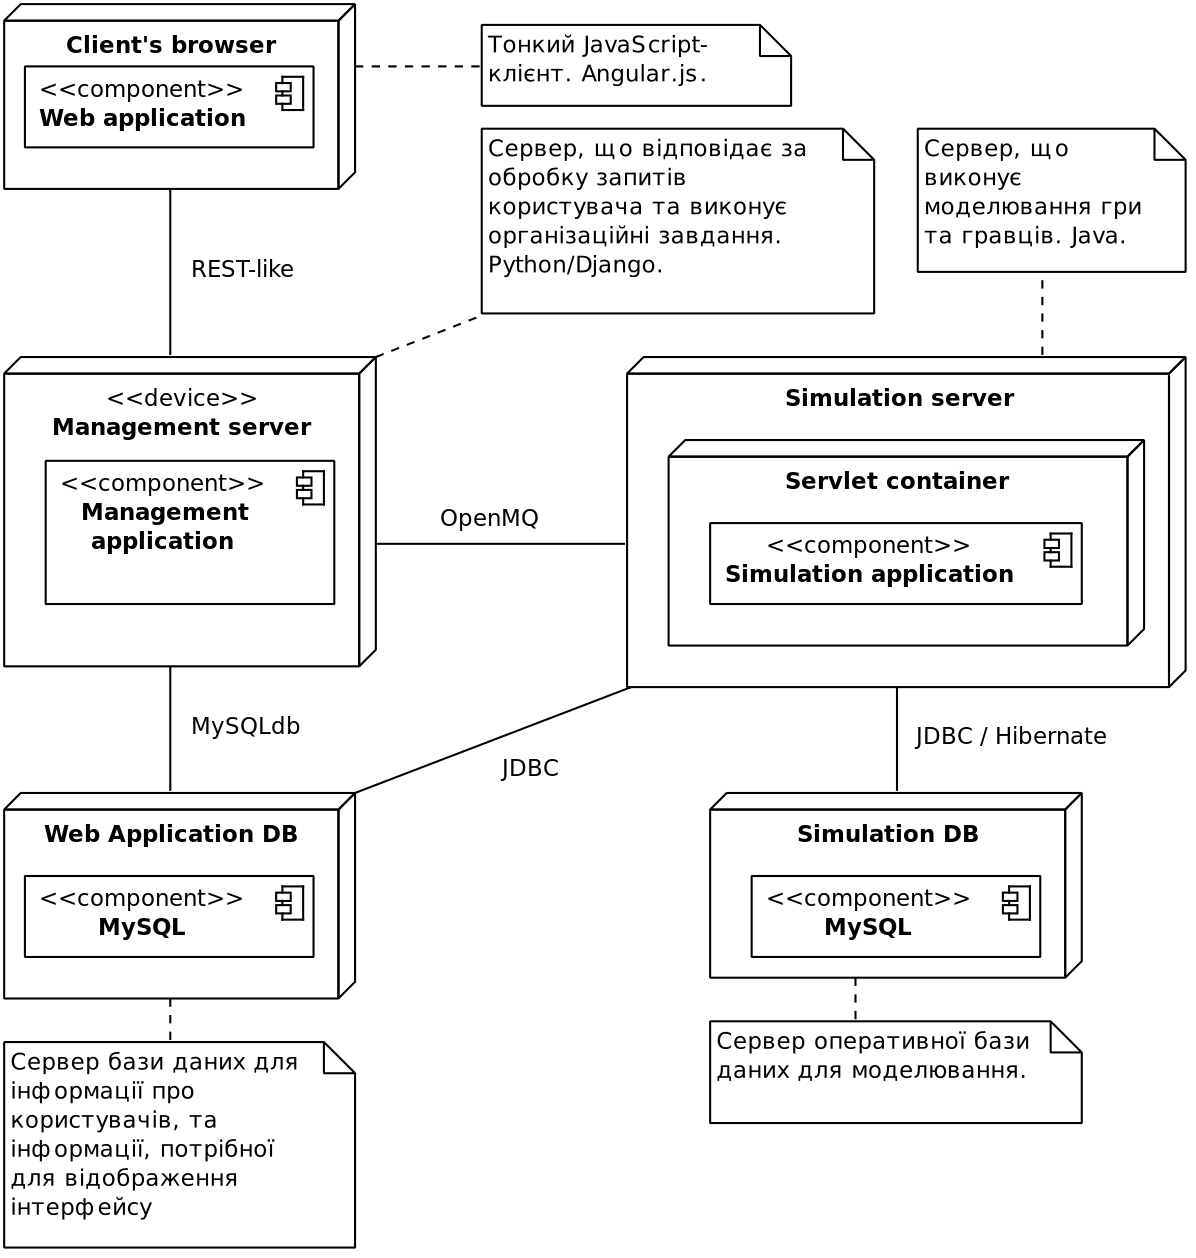
\includegraphics[width=5in]{images/uml/component_diagram.png}
    \caption{Діаграма компонентів}
    \label{fig:uml_components}
\end{stdfigure}   



\subsection{Алгоритмічне забезпечення}


\begin{stdfigure}
    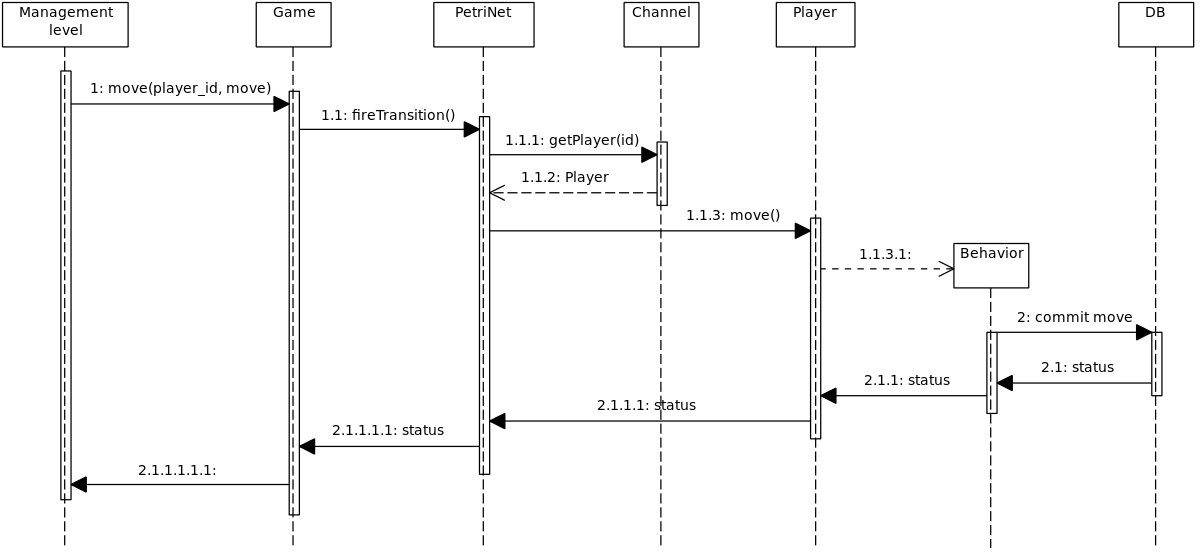
\includegraphics[width=7in]{images/uml/live_move.png}
    \caption{Діаграма послідовностей ходу реального гравця}
    \label{fig:uml_live_move}
\end{stdfigure}   

\begin{stdfigure}
    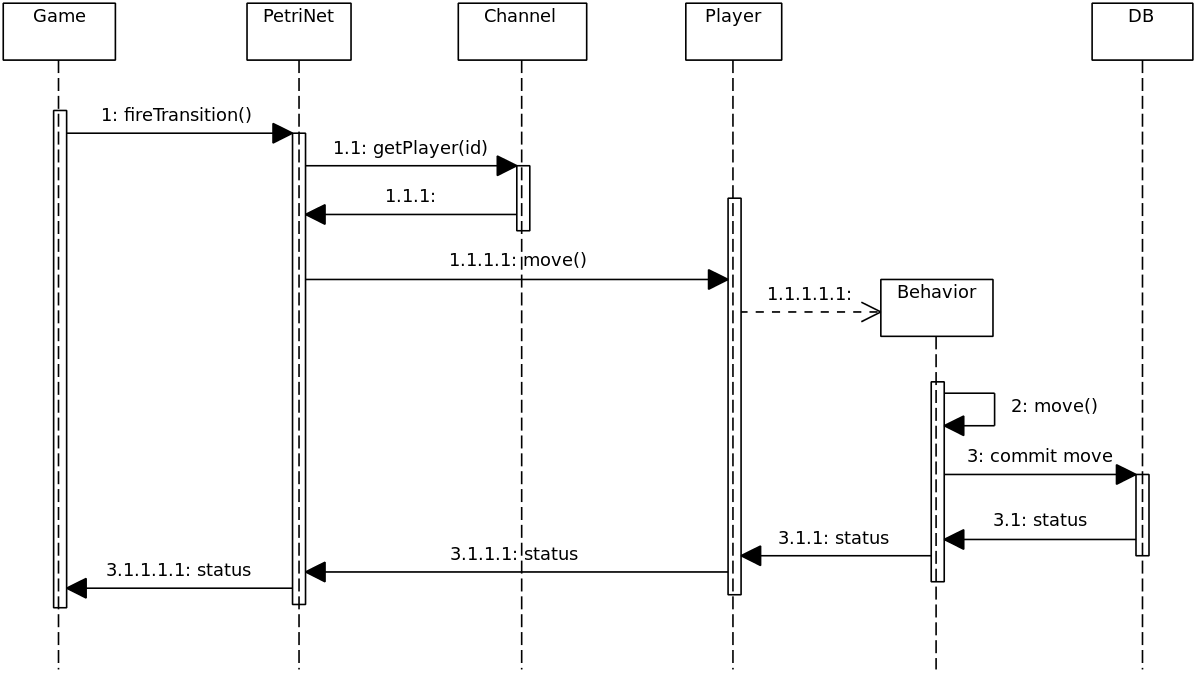
\includegraphics[width=7in]{images/uml/automate_move.png}
    \caption{Діаграма послідовностей ходу автоматичного гравця}
    \label{fig:uml_auto_move}
\end{stdfigure}   
%3.3 Алгоритмическое обеспечение (активити диаграммы)
\subsection{Інструкція користувача}

